% This must be in the first 5 lines to tell arXiv to use pdfLaTeX, which is strongly recommended.
\pdfoutput=1
% In particular, the hyperref package requires pdfLaTeX in order to break URLs across lines.

\documentclass[11pt]{article}

% Remove the "review" option to generate the final version.
\usepackage{acl}

% Standard package includes
\usepackage{times}
\usepackage{latexsym}

% Custom package includes
\usepackage{easyReview}
\usepackage{booktabs}
\usepackage{array}
\usepackage{multirow}

% Custom commands
\newcommand\MyBox[1]{
  \fbox{\lower0.75cm
    \vbox to 1.7cm{\vfil
      \hbox to 1.7cm{\hfil\parbox{1.4cm}{#1}\hfil}
      \vfil}%
  }%
}

% For proper rendering and hyphenation of words containing Latin characters (including in bib files)
\usepackage[T1]{fontenc}
% For Vietnamese characters
% \usepackage[T5]{fontenc}
% See https://www.latex-project.org/help/documentation/encguide.pdf for other character sets

% This assumes your files are encoded as UTF8
\usepackage[utf8]{inputenc}

% This is not strictly necessary, and may be commented out,
% but it will improve the layout of the manuscript,
% and will typically save some space.
\usepackage{microtype}

\usepackage{graphicx}


% If the title and author information does not fit in the area allocated, uncomment the following
%
%\setlength\titlebox{<dim>}
%
% and set <dim> to something 5cm or larger.

\title{Perceptions and Sentiments Towards the Future of AI - Deep Learning on Internet Archive Data}

% Author information can be set in various styles:
% For several authors from the same institution:
% \author{Author 1 \and ... \and Author n \\
%         Address line \\ ... \\ Address line}
% if the names do not fit well on one line use
%         Author 1 \\ {\bf Author 2} \\ ... \\ {\bf Author n} \\
% For authors from different institutions:
% \author{Author 1 \\ Address line \\  ... \\ Address line
%         \And  ... \And
%         Author n \\ Address line \\ ... \\ Address line}
% To start a seperate ``row'' of authors use \AND, as in
% \author{Author 1 \\ Address line \\  ... \\ Address line
%         \AND
%         Author 2 \\ Address line \\ ... \\ Address line \And
%         Author 3 \\ Address line \\ ... \\ Address line}

\author{
    Dünya Baradari\\Leipzig University\And
    Finn Bartels\\Leipzig University\And
    Artur Dewald\\Leipzig University\And
    Julia Peters\\Leipzig University
}

\begin{document}
\maketitle
\begin{abstract}
This document is a supplement to the general instructions for *ACL authors.
It contains instructions for using the \LaTeX{} style files for ACL conferences.
The document itself conforms to its own specifications, and is therefore an example of what your manuscript should look like.
These instructions should be used both for papers submitted for review and for final versions of accepted papers.
\end{abstract}

\graphicspath{
              {./figures/}
             }

\section{Introduction}

Human-like artificial intelligence (AI) has been exciting and frightening humanity since the antiquity.
Often intertwined with the concept of an artificial man, humanoid automata with the supposed capacity to answer questions and feel emotions have been present among all civilizations, including the ancient Egyptians and Greek \citep{Newquist1994}, Chinese \citep{cohen1986} and Mesopotamians \citep{unat2008}.
Yet, it has been in the past decades that the rise of computing power according to Moore’s Law\footnote{\url{https://www.britannica.com/technology/Moores-law}} has enabled a wide-scale application of AI technologies.
At the time of writing, use cases range from self-driving cars, personalization of ads in online browsing to highly complex predication tasks for protein folding \citep{jumper2021}.
\\
This rapid development of \emph{intelligent machines} in everyday life and applications has led to both hopes and fears among the general population.
\citet{cave2019} identify four dichotomous categories of excitement and fears about artificial intelligence.
These are immortality and inhumanity, ease and obsolescence, gratification and alienation and dominance and uprising (\autoref{dichotomy-categories}).
They further argue that such perceptions, which may not align with reality, can yet influence the development, regulation, and application of AI.
The encouragement of research into AI ethics by various public policy groups and governments may be a reflection of this point \citep{leslie2019}.
\\
In our work, we seek to follow up on the analysis of \citet{cave2019} and examine the views of the English-speaking online community regarding the future of artificial intelligence. We discern the most common clusters of topics that are formed around AI and the average sentiment for each topic using machine learning. To that end, we employ natural language processing (NLP) to extract and analyze statements about the future of AI from the Web Archive \citep{Deckers2022}, a collection of website snapshots which offers us data from the past \textasciitilde10 years.
We apply a pipeline integrating three models on this data.
The first model is a finetuned future model, which is able to recognize statements about the future.
This data is then fed into an existent sentiment classifier to add sentiments.
Finally, our last model assigns a topic to each sentence.
This dataset is subsequently analyzed for its the individual topic clusters.
While our analysis solely concerns artificial intelligence, our pipeline and models offer a way to study online views concerning the future for any topic. By examining the prevalence and sentiment of AI topics specifically, we hope to inform social science researchers, philosophers, and policy makers about the development of artificial intelligence in the general population’s perception, to direct efforts towards a better future with AI.

%%%%%%%%%%%%%%%%%%%%%%%%%%%%%%%%%%%%%%%%%%%%%%%%%%%%%%%%%%%%%%%%%%%%%%%%%%%%%%%%%%%%%%%%%%%%%%%%%%%%%%%%%%%%%%%%%%%%%%%%%%%%%%%
%%%%%%%%%%%%%%%%%%%%%%%%%%%%%%%%%%%%%%%%%%%%%%%%%%%%%%%%%%%%%%%%%%%%%%%%%%%%%%%%%%%%%%%%%%%%%%%%%%%%%%%%%%%%%%%%%%%%%%%%%%%%%%%
\begin{table}[t]
    \centering
    \resizebox{\columnwidth}{!}{%
    \begin{tabular}{lll}
        \toprule
        \textbf{Dichotomy} & \textbf{Hope} & \textbf{Fear} \\
        \midrule
        Immortality and  & Much longer     & Losing one's \\
        Inhumanity       & lives           & identity \\
        \addlinespace[0.7em]
        Ease and         & Life free       & Becoming \\
        Obsolescence     & of work         & redundant \\
        \addlinespace[0.7em]
        Gratification    & AI can fulfill  & Humans will become \\
        and Alienation   & one's desires   & redundant to each other \\
        \addlinespace[0.7em]
        Dominance        & AI offers power & AI will turn \\
        and Uprising     & over others     & against humans \\
        \bottomrule
    \end{tabular}
    }
\caption{\label{dichotomy-categories}
Categories of dichotomies of hopes and fears towards AI.
Based on \citet{cave2019}.
}
\end{table}
%%%%%%%%%%%%%%%%%%%%%%%%%%%%%%%%%%%%%%%%%%%%%%%%%%%%%%%%%%%%%%%%%%%%%%%%%%%%%%%%%%%%%%%%%%%%%%%%%%%%%%%%%%%%%%%%%%%%%%%%%%%%%%%
%%%%%%%%%%%%%%%%%%%%%%%%%%%%%%%%%%%%%%%%%%%%%%%%%%%%%%%%%%%%%%%%%%%%%%%%%%%%%%%%%%%%%%%%%%%%%%%%%%%%%%%%%%%%%%%%%%%%%%%%%%%%%%%

\section{Methodology}

For the realization of our concept, the following 3 objectives have to be accomplished:

\begin{enumerate}
    \item Obtaining of a sufficiently large data set with different expressions about the topic of AI.
    \item Raw data transformation into a data set that to the target schema illustrated in Table~\ref{data-schema}
    \item Creation of a visualization from which society's perceptions on different topics of AI can be extracted.
\end{enumerate}%
%
%
\textbf{Raw Data Extraction:}
Since a web archive with the corresponding data extraction pipeline is at our disposal, we utilize this one.
The data set consists of long texts.
For that reason the text must be splitted into separate sentences.
Then, sentences about AI can be ex tracted for later processing by applying Regex.
\\
\\
%
\textbf{Data Transformation:}
For later analysis, the data must be converted to required target schema, illustrated in Table~\ref{data-schema}, several challenges have to be handled within this stage.
\\
First, statements about the future must be extracted from all the expressions.
For that purpose we train a model with the ability to distinguish between statements about the future and all other types of terms.
Subsequently two further models are applied to add a sentiment and a topic to every future statement. statement.
The urls of the pages are also included in the data schema for a later consideration.
\\
Now the corresponding data set is prepared for further analysis.
\\
\\
\textbf{Analysis:}
For the analysis we start with a graphical visualization.
Therefore, we decided to group all statements according to their topics.
This way for every topic a sentiment analysis can be conducted separately.


\begin{table}
\setlength\tabcolsep{2pt} % let LaTeX compute intercolumn whitespace
\footnotesize\centering
\captionsetup{size=footnotesize}
\resizebox{\columnwidth}{!}{%
%\begin{tabular*}{\columnwidth}{@{\extracolsep{\fill}}%
%%%%%%%%%%%%%%%%%%%%%%%%%%%%%%%%%%%%%%%%%%%%%%%%%%%%%%%%%%%%%%%%%%%%%%%%%%%%%%%%%%%%%%%%%%%%%%%%%%%%%%%%%%%%%%%%%%%%%%%%%%%%%%%%%%%%%%%%%%%%%%%%%%%%%%
\begin{tabular}{
    cccc}

\hline

\textbf{statement} & \textbf{Sentiment} & \textbf{Topic} & \textbf{url} \\
\hline
AI can be a risk for many workers. & NEG & finances & ...\\
AI will definitely revolutionize games! & POS &  gaming & ...\\
... & ... & ... & ... \\
\hline
\end{tabular}}
%%%%%%%%%%%%%%%%%%%%%%%%%%%%%%%%%%%%%%%%%%%%%%%%%%%%%%%%%%%%%%%%%%%%%%%%%%%%%%%%%%%%%%%%%%%%%%%%%%%%%%%%%%%%%%%%%%%%%%%%%%%%%%%%%%%%%%%%%%%%%%%%%%%%%%
\caption{\label{data-schema}
Data schema for visualization and analysis
}
\end{table}

\section{Results}
\label{results}
Examining the distribution of sentiments, a definite majority of neutral statements (69\%) is clearly obvious.
The proportion of positive annotated statements (21\%) is about twice as large as the number of negatively annotated terms (11\%).
This implies a slight tendency to an overall positive attitude towards the future of AI (\autoref{fig:bar_sentiments}).
In figure \ref{fig:bar_topics} a domination of neutral statements is illustrated for each of the 9 topics.
With two exceptions, Gaming and Machine Human Interface, there are visibly more positive than negative statements on each topic.
\begin{figure}[t]
    \centering
    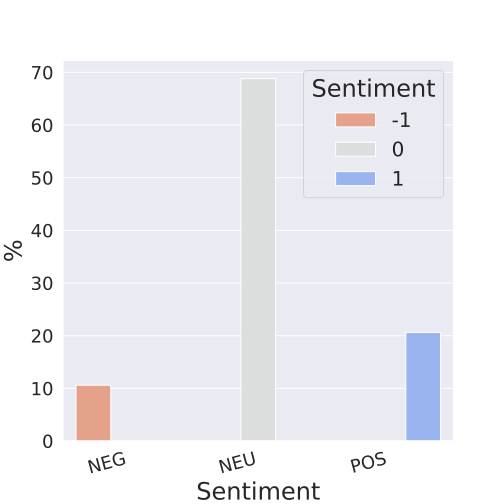
\includegraphics[width=\linewidth]{bar_sentiments}
    \caption{
        Dummy caption.
    }
    \label{fig:bar_sentiments}
\end{figure}
\\
\\
In the distribution of subtopics, we can observe a similar dominance of some subcategories.
For instance, the subcategory Data is associated with 21\% of all statements, as well as Autopilot.
Other dominant subtopics are Intelligence (19\%), Recognition (12\%), Computer (8\%) and Supercomputer (7\%) (\autoref{fig:pie_subtopics_by_occ}).
\\
\\
In the distribution of subtopics, we can observe a similar dominance of some subcategories.
For instance, the subcategory Data is associated with 21\% of all statements, as well as Autopilot.
Other dominant subtopics are Intelligence (19\%), Recognition (12\%), Computer (8\%) and Supercomputer (7\%) (\autoref{fig:pie_subtopics_by_occ}).
\\
\\
As previously described we added for sentiment of every statement.
Calculating the average the sentiment score is about 0.1.
This shows a slightly positive tendency.
The average sentiment of the most topics is majorly neutral.
The categories containing the most positive rated sentiments are Transhumanism, Natural Language Technology, and Research Computing.
The most negative sentiment on average were assigned to the categories Gaming and Search Engine.
3 of the 5 most common subtopics of Gaming have a sentiment score of less than 0 (\autoref{fig:pie_topics_subtopics_by_occ_sent_neu}).

\section{Discussion}

\subsection{Results}
Our results reveal a slightly positive outlook of people on future of AI. Interestingly, two thirds of our filtered statements were neutral, which, together with the nature of our top domain sources, suggests a large proportion of texts coming from academic or unbiased texts rather than strong opinions. The presence of about twice as many positively compared to negatively sentences and thereby a rather hopeful outlook into the future, may also be influenced by the optimism bias, which is when humans tend to overestimate the likelihood of positive events and underestimate that of negative \citep{sharot2011optimism}. These findings also align with a large-scale study made by Google researchers on the public opinion regarding the long-term impact of AI on society (Kelley et al., 2021). This study, which surveyed people from eight English and non-English speaking countries, shows a clear dominance of neutral perceptions in English-speaking countries (USA: 53\%, Australia: 57\%, Canada: 56\%) and a greater proportion of positive sentiments (USA: 21\%, Australia: 18\%, Canada: 20\%) than negative (USA: 17\%, Australia: 14\%, Canada: 15\%). Intriguingly, respondents from emerging economies such as Brazil, India and Nigeria exhibit far more optimistic opinions on the future of AI (BR: 38\%, IN: 51\%, NI: 37\%), a finding that has been repeatedly confirmed in a recent survey by the World Economic Forum \citep{Markovitz2022}. This difference may be due to these countries’ younger and generally more optimistic population, which may view AI as an essential opportunity for leapfrogging \citep{zhenmin2019frontier}. While we filtered our statements for English-speaking websites only, the prevalence of English as the world’s lingua franca must have led to the inclusion of opinions and statements from non-English speaking people. This may explain the slight skew towards positive sentiments in our data compared to sentiments from the USA, Australia and Canada from \citet{kelley2021exciting}.
Comparing our topic clusters with the dichotomies of hopes and fears by \citet{cave2019}, we can only find a weak overlap between the data. Machine human interface and transhumanism well match the authors’ first category of Immortality and Inhumanity. Interestingly, all subtopics within these clusters were labelled either neutral or positive, with those from transhumanism even displaying the most positive sentiments. The only subtopic receiving a negative label when compared to the overall sentiment mean of 0.1 (Appendix XXX) is autopilot from the machine human interface cluster, suggesting the main concern to be losing conscious control by the use of such interfaces in the future. From this, we conclude a disproportionate number of opinions in favor of transhumanism and a machine-enabled future in relation to opinions highlighting the possible (existential) risks and dangers to our “human” identity. The Natural language technology cluster in turn may point towards applications of such technologies that make life easier, such as Amazon’s Alexa, thereby fitting the category of Ease and possibly Gratification. Yet, the corresponding counterparts in the dichotomies are hard to find in our clusters, where the only negatively labelled subtopics exist in the gaming cluster. This aspect can be explained by the increasing prevalence of AI-mediated systems in games, from non-playable characters (which can include enemies, a highly negative subtopic) to iterative game improvement and graphical enhancement \citep{anandrise}. While the latter two examples provide advantages for the gamer, it may be that the idea of an AI as the enemy predominates since this is the primary noticeable direct touchpoint between the user and an AI. 
Furthermore, there are no clusters that we consider well-fitting for \citet{cave2019} category Dominance and Uprising, which, curiously, is a category commonly discussed by popular figures such as the late Stephen Hawking \citep{hawking2014transcendence}. Overall, it rather that our clusters center around applications of artificial intelligence. This is further demonstrated by the fact that several subtopics repeat within clusters (Figure XXX). For instance, “autopilot” is present within the machine human inference, natural language processing, finance, search engine, social media, and transhumanism clusters. Other repeated subtopics include data, supercomputer, computer, intelligence, recognition, and machine. Together with the slightly positive but largely neutral overall sentiment, which suggests that people speak mainly rationally about the future of AI, we reason that discussions center primarily around areas of application of AI technology instead of opinionated positions about its benefits and risks. 

\subsection{Topic Assignment}
\label{topics}
As described in section \ref{results} the most statements are assigned with the "machine human interface" topic.
This is not surprising, since technical sources clearly dominate our websites. 
Technological systems often require human operation and contain a corresponding interface as an implicit feature.
Also search engines often need the handling from the outside. 
For this reason, many of these search engine related phrases end up in this category instead of in the search engine topic.
Since search engines also correspond to natural language systems, they are often assigned to the category "natural language technology".
To avoid this, more distinct generic terms for topics should have been chosen.
This issue also arises in the field of "human machine interface". 
Statements that describe a friendly AI are grouped in this category . 
We would expect this kind of sentences in "transhumanism".
The reason for this could be the categpry name, since it combines the terms human and machine.
\\
"Computer vision", "natural language technology", "social media", "transhumanism" and "human machine interface" contain many statements that do not fit the corresponding topic.
Whereas this appears quite random for "natural language technology" and "human machine interface", since we did not define suitable topics for these sentences.
In "computer vision" many sentences end up containing words like scan, look, see.
But these do not actually refer to the topic.
Similarly "social media" includes  statements with the word fans, even if this sentence is about attending a soccer match.
But also in this category are plenty of randomly assigned statements.
Nevertheless, the categories "computer vision" and "natural language technology" also contain appropriate phrases.  
The quality of these subjects is mixed.
"human machine interface" consists of far too many terms that do not fit to this topic. 
A possible solution for such random assignments could be to add the generic category "others".
Furthermore, it should be considered whether the category human machine interface is actually useful.
It does not seem specific enough to narrow down a particular topic.
\\
The Topic Model seems to assign the "research computing" category to statements more reliably.
Nevertheless, it is noticeable that educational topics that cannot be associated with research and hardware or software are also grouped under this theme.
Sentences regarding technical topics, which have no connection with research, also often fall into this category.
However, in the end it is a matter of interpretation whether these statements do not fall under "research computing".
\\
Finally, there are also topics that seem to be correctly assigned to their statements for the majority of the time.
The corresponding categories are finance and gaming.
This could be an indication that the model is not suitable for too specific technical terms.
Providing more common topics contained in the everyday english language use, could result in a more reliable topic annotation.
\subsection{Website Examination}

The final data set, produced by the model pipeline, contains the url for every AI future statement.
Table~\ref{Top-Domains} presents the domains that are mostly occurring in this final data set.
When examining the main domains, these appear relatively  diversified.
A website dealing with phylosophical questions on the topic of AI is included (lesswrong.com).
Following this, there are three sites from the field of gaming (acceleratingfuture.com, mugenguild.com, slightlymagic.net).
Also, the blog of the department of defense is contained among these domains dealing with the research of defence and military needs (dodsbir.net).
A store with speech recognition devices is also available (knowbrainer.com).
Nevertheless a number of scientific blogs on AI-related topics are also include, which are lead by researchers or from the tech industry.
Latter are mostly data scientists.
Considering the other domains, many scientific websites as well as websites about gaming are also very abundant.
Thus, rather the future statements were expressed by people from AI related fields.
This could mean that this topic has a lower role in the general population and thus it is dealt very little with AI-specific topics in the public society.
New discoveries could be made by observing domains containing statements from the last few months were used.
More people might feel affected by the latest developments in this area.
Consequently, there could be more blogs with people from other sectors who would exchange opinions about these developments.
%%%%%%%%%%%%%%%%%%%%%%%%%%%%%%%%%%%%%%%%%%%%%%%%%%%%%%%%%%%%%%%%%%%%%%%%%%%%%%%%%%%%%%%%%%%%%%%%%%%%%%%%%%%%%%%%%%%%%%%%%%%%%%%%%%%%%%%%%%%%%%%%%%%%%%
%%%%%%%%%%%%%%%%%%%%%%%%%%%%%%%%%%%%%%%%%%%%%%%%%%%%%%%%%%%%%%%%%%%%%%%%%%%%%%%%%%%%%%%%%%%%%%%%%%%%%%%%%%%%%%%%%%%%%%%%%%%%%%%%%%%%%%%%%%%%%%%%%%%%%%
\begin{table}
    \setlength\tabcolsep{2pt} % let LaTeX compute intercolumn whitespace
    \centering
    \captionsetup{size=footnotesize}
    \resizebox{\columnwidth}{!}{%
    %\begin{tabular*}{\columnwidth}{@{\extracolsep{\fill}}%
    %%%%%%%%%%%%%%%%%%%%%%%%%%%%%%%%%%%%%%%%%%%%%%%%%%%%%%%%%%%%%%%%%%%%%%%%%%%%%%%%%%%%%%%%%%%%%%%%%%%%%%%%%%%%%%%%%%%%%%%%%%%%%%%%%%%%%%%%%%%%%%%%%%%%%%
    \begin{tabular}{rll}
        \toprule
        \textbf{AI statements} & \textbf{Website} & \textbf{Description} \\
        \midrule
        \multirow{2}{*}{210\quad} & \multirow{2}{*}{lesswrong.com}          & Philosophical blog \\
                                  &                                         & about AI developments \\
        \addlinespace[0.7em]
        \multirow{2}{*}{198\quad} & \multirow{2}{*}{arcengames.com}         & Page of an indie \\
                                  &                                         & game developer \\
        \addlinespace[0.7em]
        \multirow{2}{*}{182\quad} & \multirow{2}{*}{acceleratingfuture.com} & Blog about perspectives \\
                                  &                                         & and emerging technologies \\
        \addlinespace[0.7em]
        \multirow{2}{*}{156\quad} & \multirow{2}{*}{heatonresearch.com}     & Blog of a data \\
                                  &                                         & scientist \\
        \addlinespace[0.7em]
        \multirow{2}{*}{106\quad} & \multirow{2}{*}{dodsbir.net}            & Research blog of the \\
                                  &                                         & department of defense \\
        \addlinespace[0.7em]
        \multirow{2}{*}{76\quad}  & \multirow{2}{*}{kdnuggets.com}          & Blog of data scientists for \\
                                  &                                         & analytics and machine learning \\
        \addlinespace[0.7em]
        \multirow{2}{*}{71\quad}  & \multirow{2}{*}{knowbrainer.com}        & Shop containing speech \\
                                  &                                         & recognition devices\\
        \addlinespace[0.7em]
        {58\quad}                 & mugenguild.com                          & 2D fighting game \\
        \addlinespace[0.7em]
        {52\quad}                 & aidreams.co.uk                          & Robotics and AI blog\\
        \addlinespace[0.7em]
        \multirow{2}{*}{51\quad}  & \multirow{2}{*}{slightlymagic.net}      & Rules Engine for the game \\
                                  &                                         & ``Magic: the Gathering'' \\
        \bottomrule
    \end{tabular}
    }
\caption{\label{Top-Domains}
Top Domains
}
\end{table}
%%%%%%%%%%%%%%%%%%%%%%%%%%%%%%%%%%%%%%%%%%%%%%%%%%%%%%%%%%%%%%%%%%%%%%%%%%%%%%%%%%%%%%%%%%%%%%%%%%%%%%%%%%%%%%%%%%%%%%%%%%%%%%%%%%%%%%%%%%%%%%%%%%%%%%
%%%%%%%%%%%%%%%%%%%%%%%%%%%%%%%%%%%%%%%%%%%%%%%%%%%%%%%%%%%%%%%%%%%%%%%%%%%%%%%%%%%%%%%%%%%%%%%%%%%%%%%%%%%%%%%%%%%%%%%%%%%%%%%%%%%%%%%%%%%%%%%%%%%%%%
\subsection{Project Limitations}

Since we had a limited time for this project, there are some aspects where we would have liked to continue our work.
From a technical point of view, we would have preferred to spend additional time on labelling more data for the sentiment model.
Thus, it could have been possible to finetune this model as well.
With our current approach, we only keep the AI future predictions if the sentiment model makes a prediction with a certainty of more than 70\%.
This results in the loss of a few additional statements that we would have available for analysis.
\\
Investing more time in topic selection would also be beneficial.
Therefore, it might be reasonable to manually evaluate our statements with the corresponding topics with a subsequent performing of a another topic selection.
Furthermore, better results can be achieved by finetuning the topic model.
\\
Unfortunately, the location containing the corresponding date on the website does not contain the corresponding date is not consistent.
Accordingly, we would have needed more time for the date extraction.
Providing a year for each statement could illustrate how the perception of a certain topic in the field of AI has changed over time.
Having insights about such trends, allows monitoring the developments in cultural perceptions over time periods.
\\






\section{Conclusion}
While other groups have previously assessed the perception of AI technologies of certain groups of people, such as investors \citep{manrai2022investor}, librarians \citep{hervieux2021perceptions}, and healthcare professionals \citep{castagno2020perceptions}, or assessed perceptions at current \citep{sankaran2021exploring}, we present the first study to our knowledge that infers people’s feelings towards different areas of AI in the future from online sources. 
The public perception of this technology plays an important part in its development for it influences R\&D funding, adoption, and regulation. \\
Our findings show a slightly positive perception of the future of AI by the English-speaking online community of the past 10 years. Topic-wise, web content seems to deal primarily with areas of application of AI, which, together with the near-neutral average sentiment may suggest a rather matter-of-facts approach in which people have been thinking and writing about AI’s future.
Our approach consists of a pipeline to filter statements about the future and label them with their appropriate sentiments and topics.
In concert, our method offers researchers a way of analyzing statements for opinions and topics in regards to the future for not only artificial intelligence but any subject.

% Entries for the entire Anthology, followed by custom entries
\bibliography{anthology,custom}

\onecolumn
\appendix
\section{Data Set Card: Future Statements}
\\
\\
\textbf{Data Set Description}
\\
\\
This Data Set Card originates from \url{https://huggingface.co/datasets/fidsinn/future-statements}
The english language data set contains 2,500 statements.
50\% of the relate to future events and 50\% of which relate to non-future events.
The statements were collected manually and programmatically from several websites and datasets.
The labels were set manually or programmatically (including corresponding manual examination of the labels).
\\
\\
\textbf{Dat Set Motivation}
\\
\\
The sole purpose of this dataset was to fine tune the distilbert-base-uncased \url{https://huggingface.co/distilbert-base-uncased} model into our distilbert-base-future \url{https://huggingface.co/fidsinn/distilbert-base-future} model.
The dataset was created by students from the University of Leipzig in the Big Data and Language Technologies Module of the Webis Group \url{https://huggingface.co/webis}.
\\
\\
\textbf{Data Set Composition}
\\
\\
The instances are represented by single-/ or multi-sentence statements from following sources (unequally distributed):
%
\begin{itemize}
    \item \url{http://www.kaggle.com/unitednations/un-general-debates}
    \item \url{http://data.world/ian/united-nations-general-debate-corpus}
    \item \url{http://gadebate.un.org/}
    \item \url{http://dataverse.harvard.edu/dataset.xhtml?persistentId=doi:10.7910/DVN/0TJX8Y}
    \item \url{http://www.wsj.com/}
    \item \url{http://www.vox.com/}
    \item \url{http://futechblog.com/}
    \item \url{http://www.weforum.org/}
    \item \url{http://wired.com/}
    \item \url{http://openai.com/blog/}
    \item \url{http://techcrunch.com/}
    \item \url{http://futurism.com}
\end{itemize}
%
- The dataset consists of 2,500 statements in total, 50\% of which relate to future events and 50\% of which relate to non-future events.
\\
\\
\textbf{Data Set Annotation}
%The label is represented by the 'future'-column:
\begin{itemize}
    \item 0: No future statement
    \item 1: future statement
\end{itemize}%
\\
\\
\textbf{Noise, Biases and Redundancies}
\\
\\
The main goal of the data collection process was to find future statements and general statements in equal amount.
The thematic content within the statements can be redundant and some topics can be much more present.
The dataset was not created to work with the thematic content while only fine-tune an already existing model into a model which is sensible for future and non-future statements.
Data in the 'statement'-column is publicly available and does not contain confidential information.
It was collected in the months 06/2022-07/2022 but the content of the dataset is independent of the data collection period and can be from earlier periods.
\\
\\
\textbf{Data Set Collection Process}
\\
\\
The data is directly observable on the websites mentioned in upper section.
It was collected manually and programmatically (using Pythons NLTK library for automatic sentence-extraction and Regex-filtering)
from graduate students D. Baradari \url{https://huggingface.co/Dunya}, F. Bartels \url{https://huggingface.co/fidsinn}, A. Dewald, J. Peters \url{https://huggingface.co/jpeters92} as part of a data science module of the University of Leipzig.
The data was obtained in the months 06/2022-07/2022 but the content of the dataset is independent of the data collection period and can be from earlier periods.
\\
\\
\textbf{Dataset Maintenance}
\\
\\
Curators of the dataset can be contacted via the Huggingface community tab \url{https://huggingface.co/datasets/fidsinn/future-statements/discussions}.

It is not planned to update the dataset for further work or investigations.
\section{Model Card: Future Statement Model}
This model is a finetuned on 2500 expressions, which contained 1250 future statements. distilbert-base-uncased serves as a base model
\\
\\
%
\textbf{Model Description}
%
\begin{itemize}
    \item Huggingface name: distilbert-base-future
    \item Creation Date: 11/08/22
    \item Version: 1.0
    \item model type: text classification
\end{itemize}%
%
\textbf{Intended Use \& Limitations}
%
\begin{itemize}
    \item The primary intended use is the classification of input into a future or non-future sentence/statement.
    \item The model is primarily intended to be used by researchers to filter or label a large number of sentences according to the grammatical tense of the input.
\end{itemize}%
%
\textbf{Hyperparameters}
\\
\\
The following hyperparameters were used during training
\begin{itemize}
    \item optimizer:
    name: Adam, learning\_rate: 5e-05, decay: 0.0, beta\_1: 0.9, beta\_2: 0.999, epsilon: 1e-07, amsgrad: False
    \item training\_precision: float32
\end{itemize}%
\label{sec:appendix}
%
\textbf{Training Results}
\\
For finetuning, we have 80\% of of records from our self-annotated future-tatements dataset. This corresponds to 2000 records.
The remaining 500 will be used to test the final distilbert-base-future model
\\
%%%%%%%%%%%%%%%%%%%%%%%%%%%%%%%%%%%%%%%%%%%%%%%%%%%%%%%%%%%%%%%%%%%%%%%%%%%%%%%%%%%%%%%%%%%%%%%%%%%%%%%%%%%%%%%%%%%%%%%%%%%%%%%%%%%%%%%%%%%%%%%%%%%%%%
%%%%%%%%%%%%%%%%%%%%%%%%%%%%%%%%%%%%%%%%%%%%%%%%%%%%%%%%%%%%%%%%%%%%%%%%%%%%%%%%%%%%%%%%%%%%%%%%%%%%%%%%%%%%%%%%%%%%%%%%%%%%%%%%%%%%%%%%%%%%%%%%%%%%%%
\begin{table}[ht]
    \scriptsize
    \setlength\tabcolsep{10pt} % let LaTeX compute intercolumn whitespace
    \footnotesize\centering
    \begin{tabular}{ccccc}
        \toprule
        \textbf{Epoch} & \textbf{Train Loss} & \textbf{Train Accuracy} & \textbf{Val. Loss} & \textbf{Val. Accuracy} \\
        \midrule
        0 & 0.3816 & 0.8594 & 0.1547 & 0.9475 \\
        1 & 0.1142 & 0.9613 & 0.1272 & 0.9625 \\
        \bottomrule
    \end{tabular}
    \caption{\label{future-model-train}
    Training Results
    }
\end{table}
%%%%%%%%%%%%%%%%%%%%%%%%%%%%%%%%%%%%%%%%%%%%%%%%%%%%%%%%%%%%%%%%%%%%%%%%%%%%%%%%%%%%%%%%%%%%%%%%%%%%%%%%%%%%%%%%%%%%%%%%%%%%%%%%%%%%%%%%%%%%%%%%%%%%%%
%%%%%%%%%%%%%%%%%%%%%%%%%%%%%%%%%%%%%%%%%%%%%%%%%%%%%%%%%%%%%%%%%%%%%%%%%%%%%%%%%%%%%%%%%%%%%%%%%%%%%%%%%%%%%%%%%%%%%%%%%%%%%%%%%%%%%%%%%%%%%%%%%%%%%%
%
%
\\
\textbf{Framework versions}
\begin{itemize}
    \item Transformers 4.18.0
    \item Tensorflow 2.8.0
    \item Tokenizers 0.12.1
\end{itemize}%
%
\pagebreak
\textbf{Test Set Results}
\begin{figure}[h]
    \centering
    \includegraphics[width=0.5\textwidth]{cm}
    \caption{
        Confusion matrix after applying the test set with the resulting accuracy of 93,8\%.
    }
    \label{fig:cm}
\end{figure}

\section{Remaining Figures}
\begin{figure}[h!]
    \centering
    \includegraphics[width=\textwidth]{bar_topics}
    \caption{
        Distribution of statements among the 9 topic categories divided into the assigned sentiment labels (-1:NEGATIVE, 0:NEUTRAL, 1:POSITIVE).
        A domination of neutral statements can be observed for each of the 9 topics.
        There are visibly more positive than negative statements except for Gaming and Machine Human Interface.
    }
    \label{fig:bar_topics}
    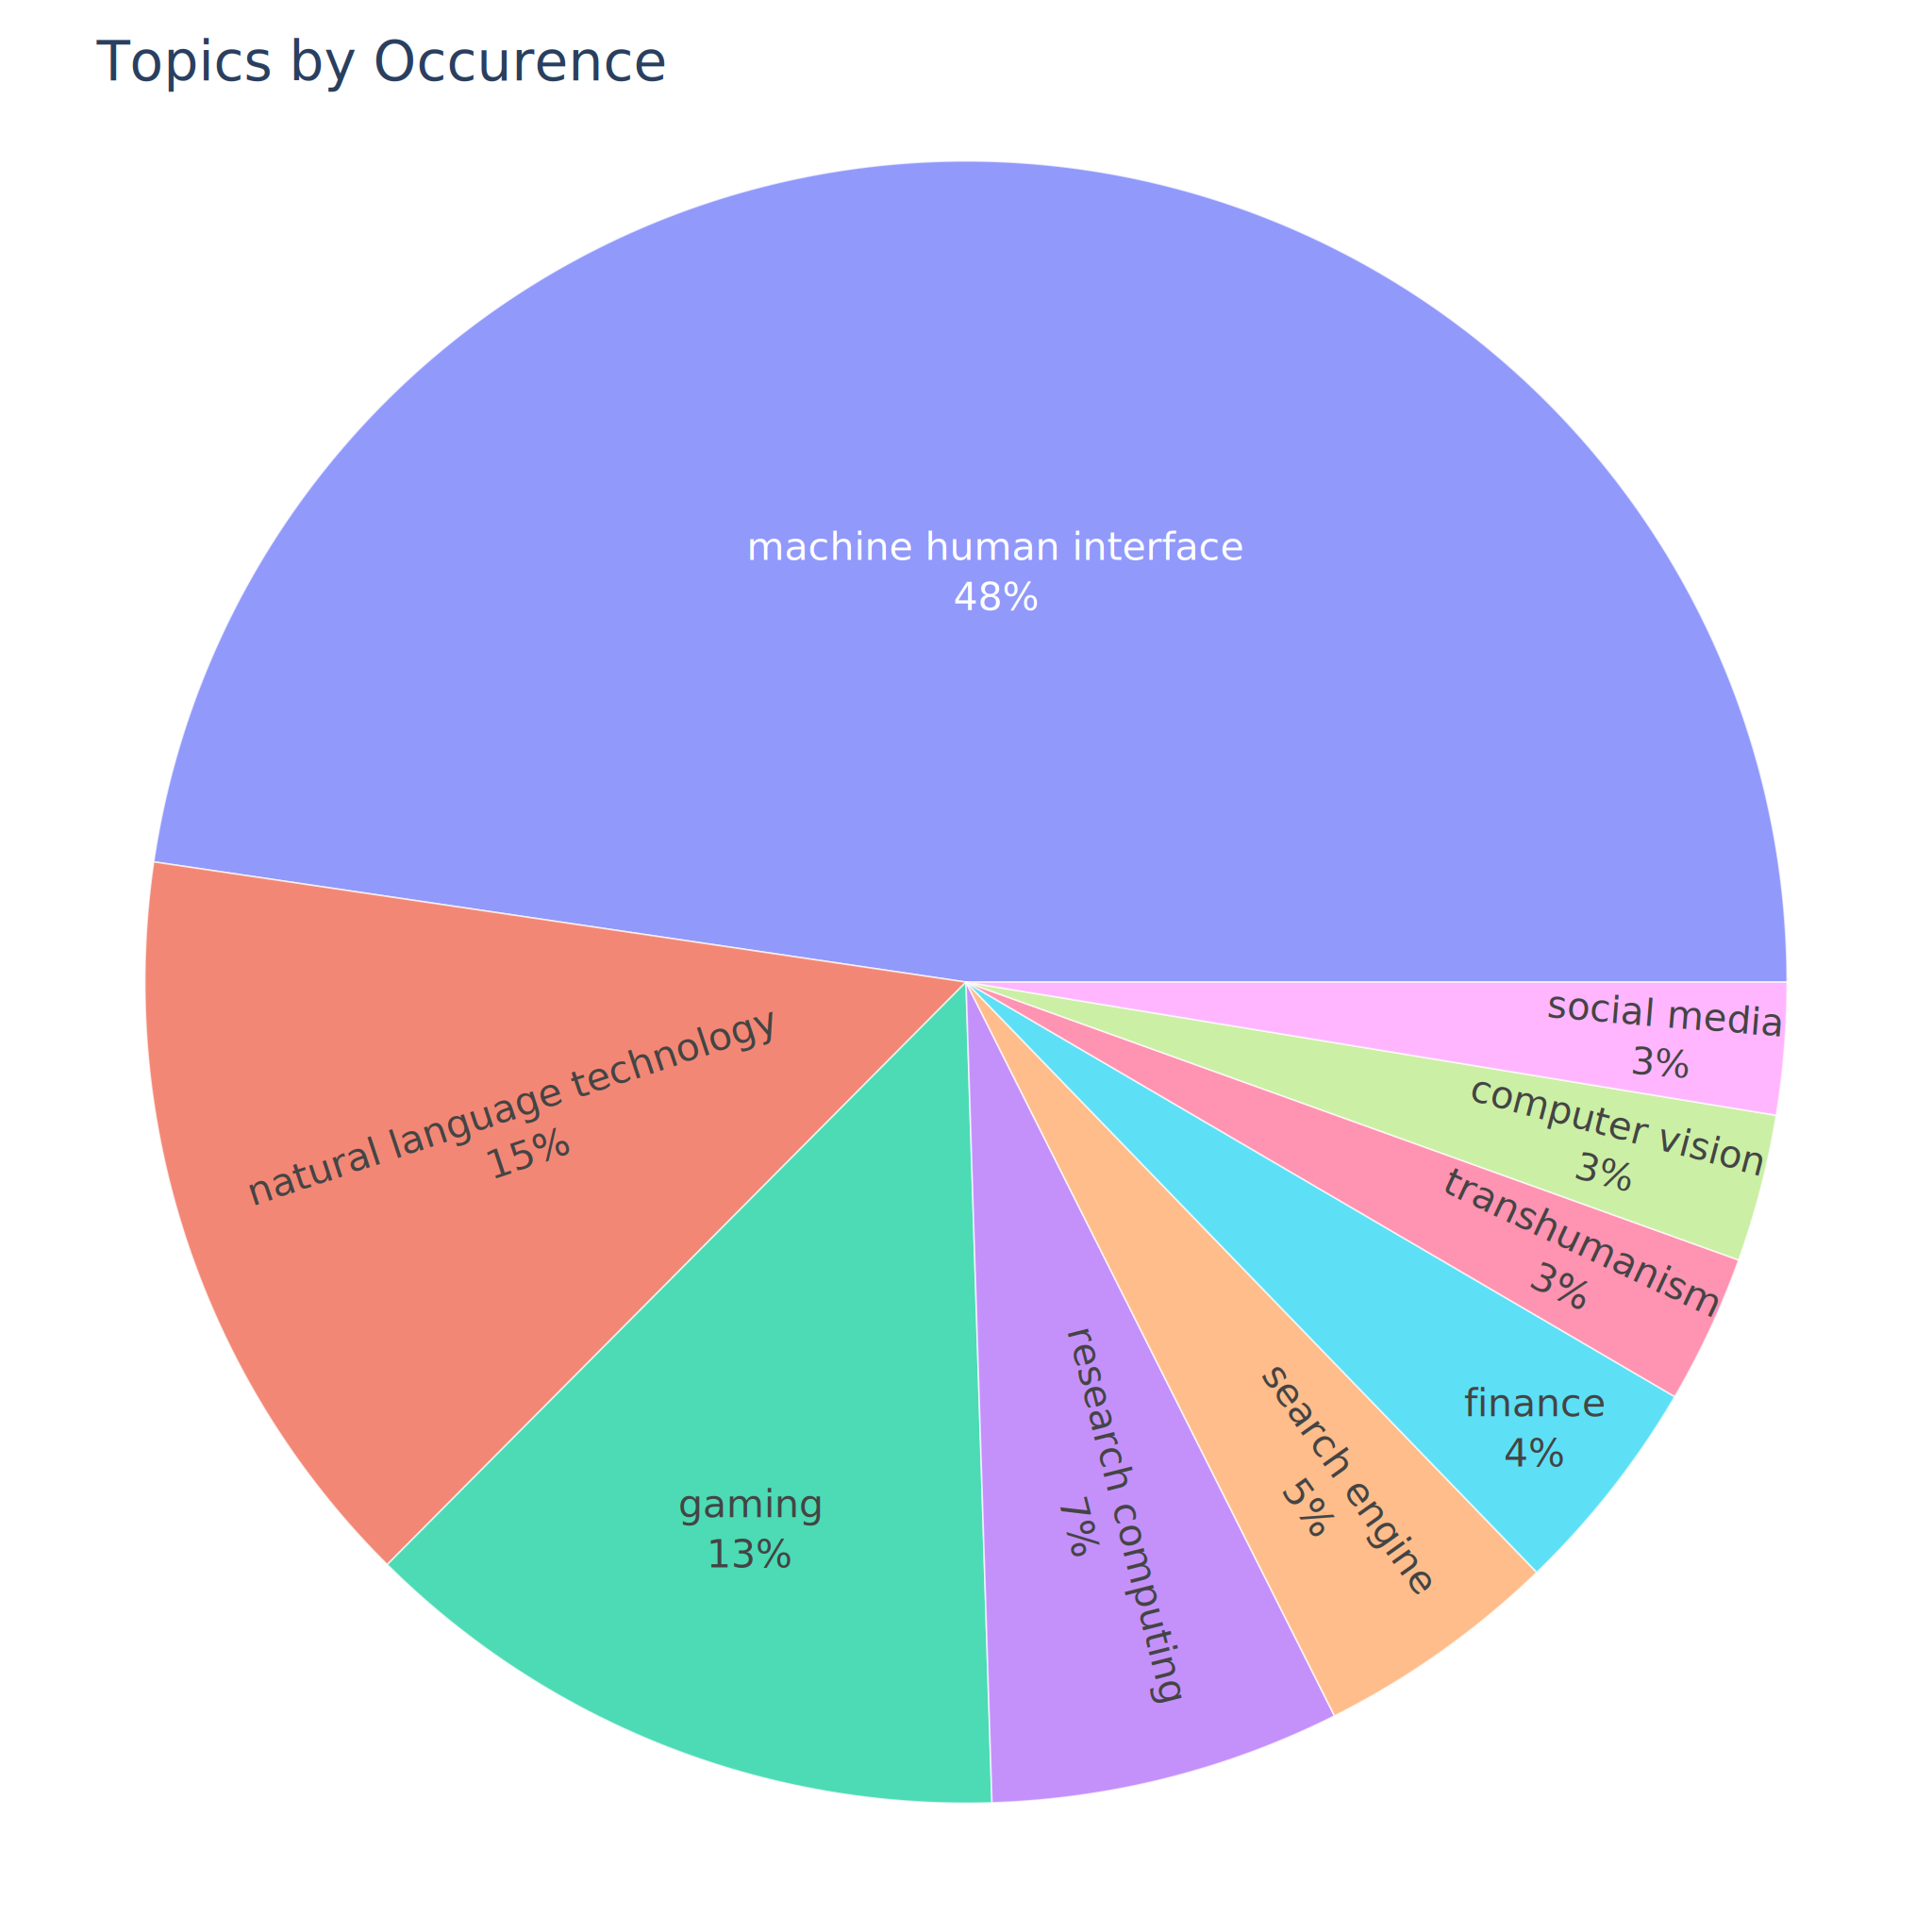
\includegraphics[width=0.6\textwidth]{pie_topics_by_occ}
    \caption{
        Distribution of statements among the 9 topic categories (in \%). 
        Statements are not equally distributed.
        Machine Human Interface describes about half of all statements (48\%).
        Gaming as well as Natural Language Technology account for about 15\% of all statements.
    }
    \label{fig:pie_topics_by_occ}
\end{figure}
\pagebreak
\begin{figure}[h!]
    \centering
    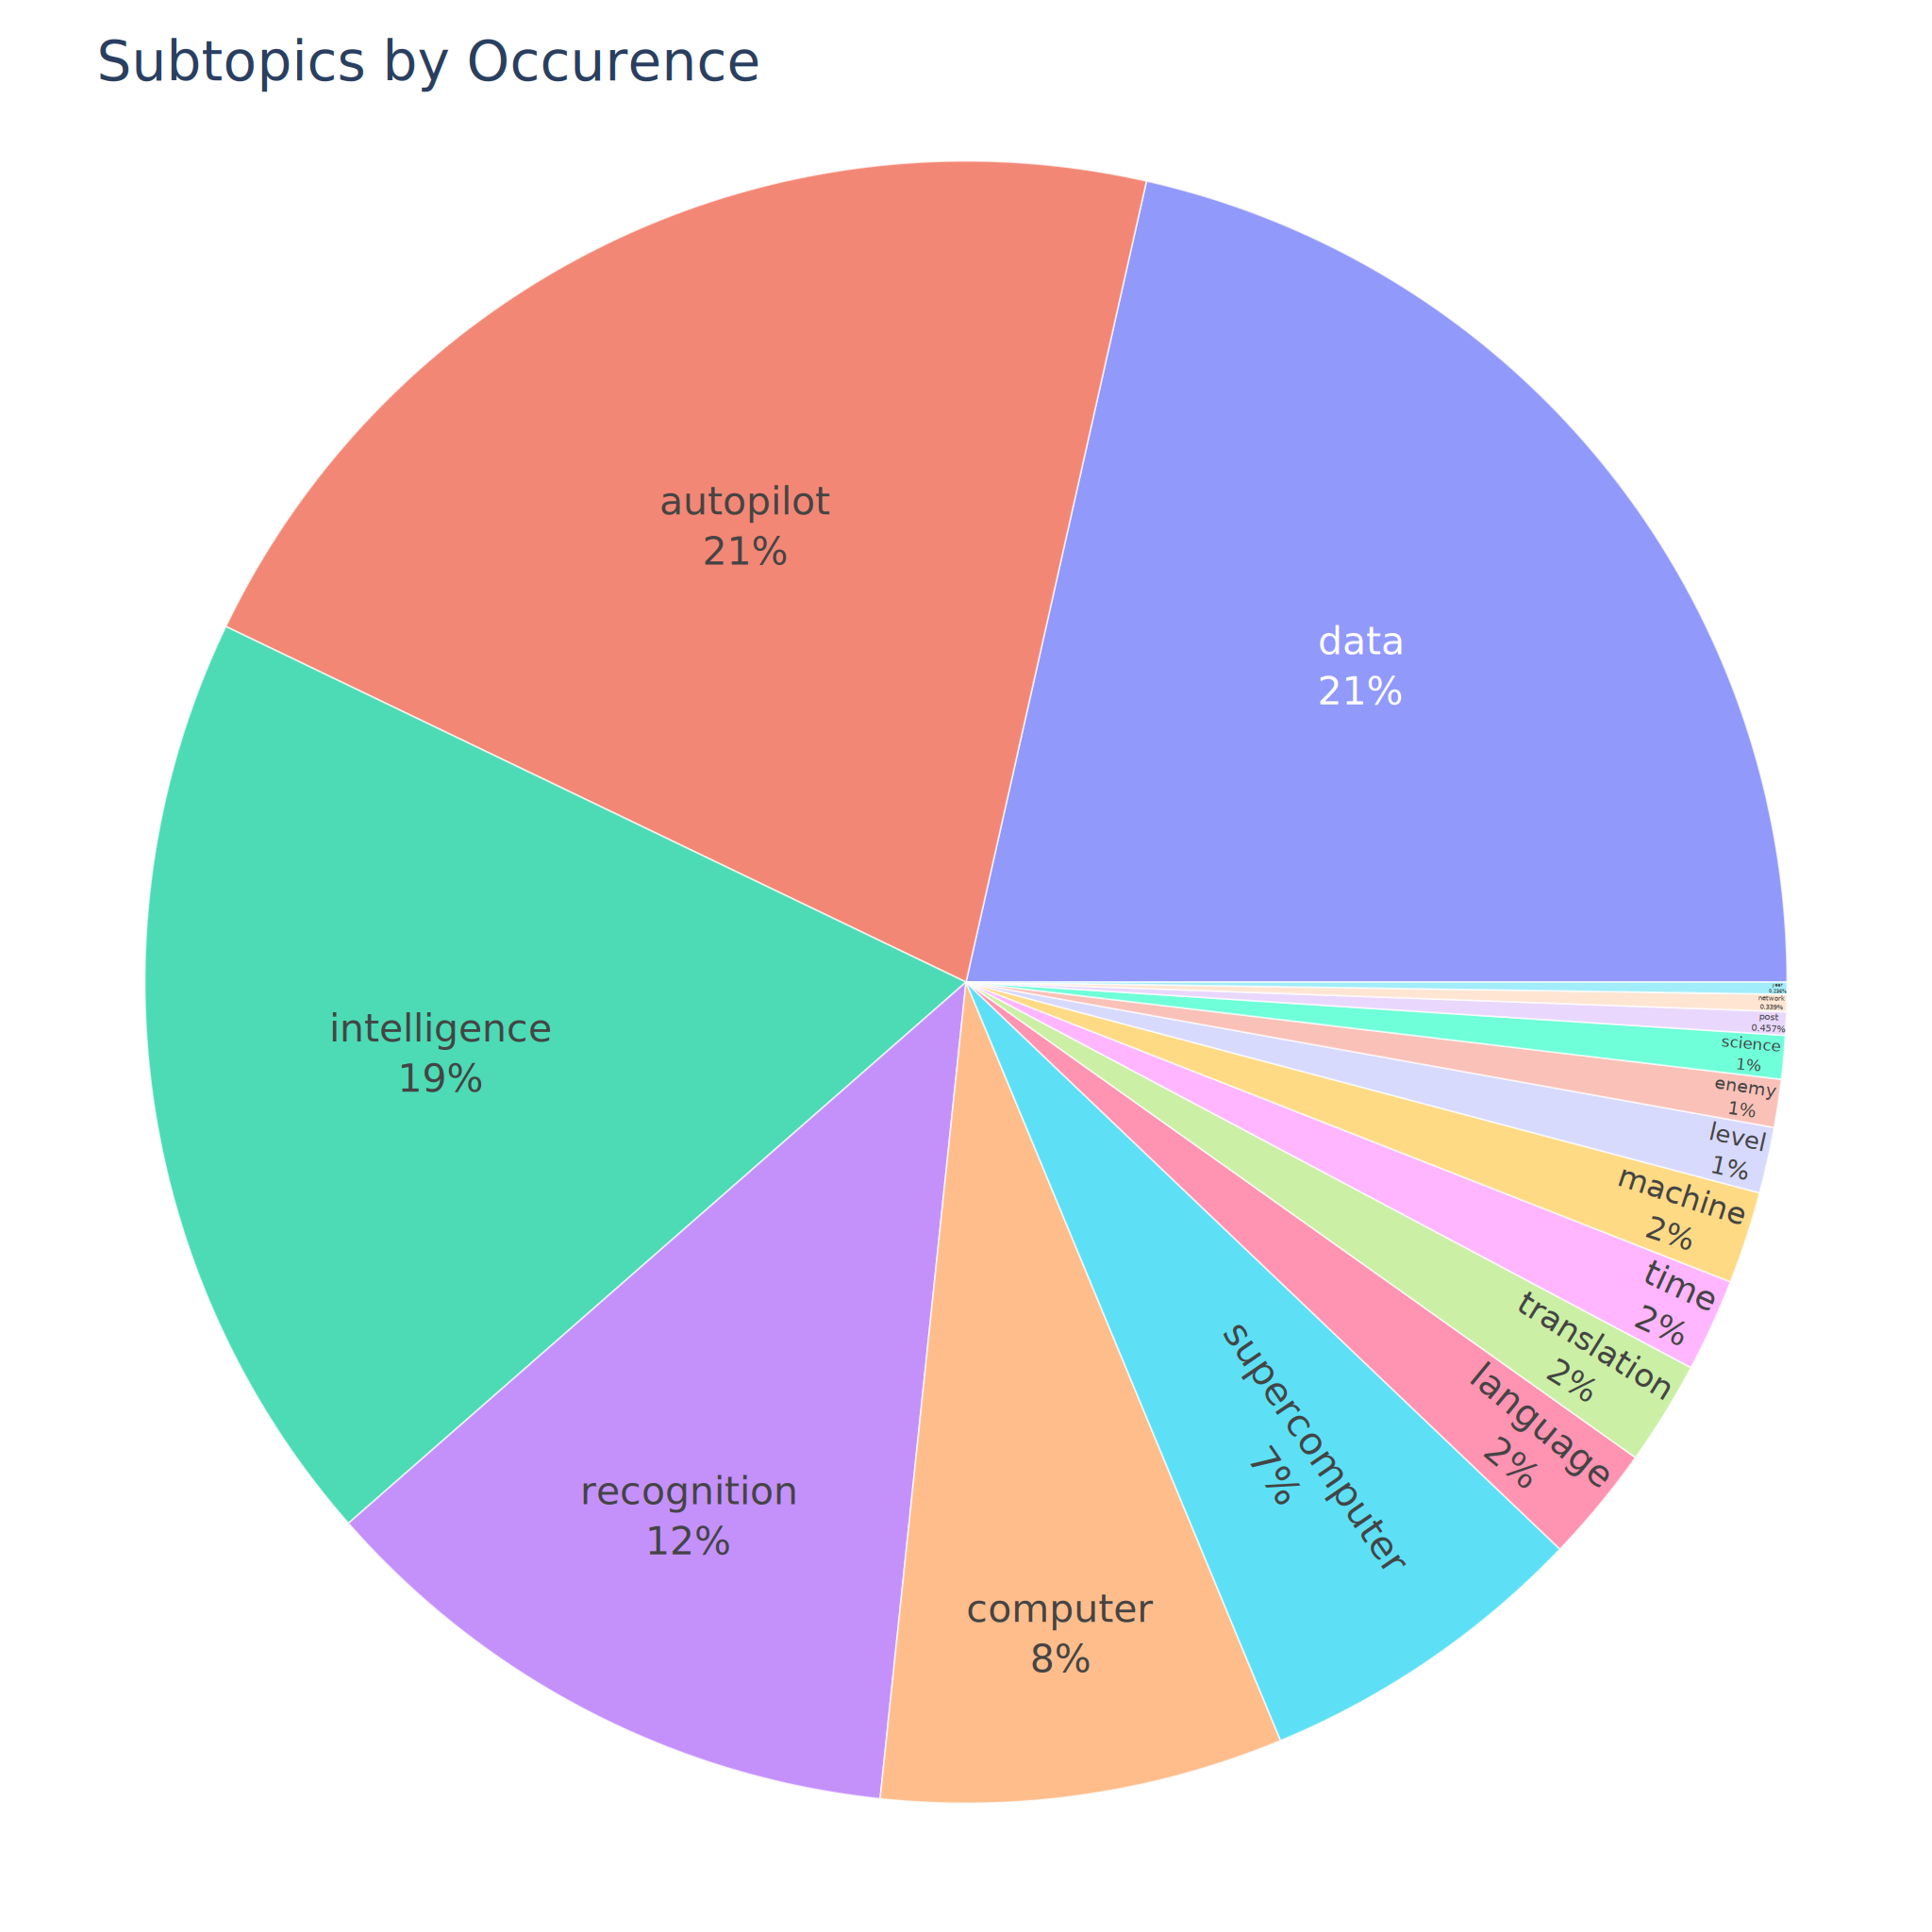
\includegraphics[width=0.6\textwidth]{pie_subtopics_by_occ}
    \caption{
        Distribution of statements among the most frequently occuring subtopic categories (in \%).
        Data (21\%), Autopilot (21\%) and Intelligence (19\%) are dominant subcategories.
    }
    \label{fig:pie_subtopics_by_occ}
    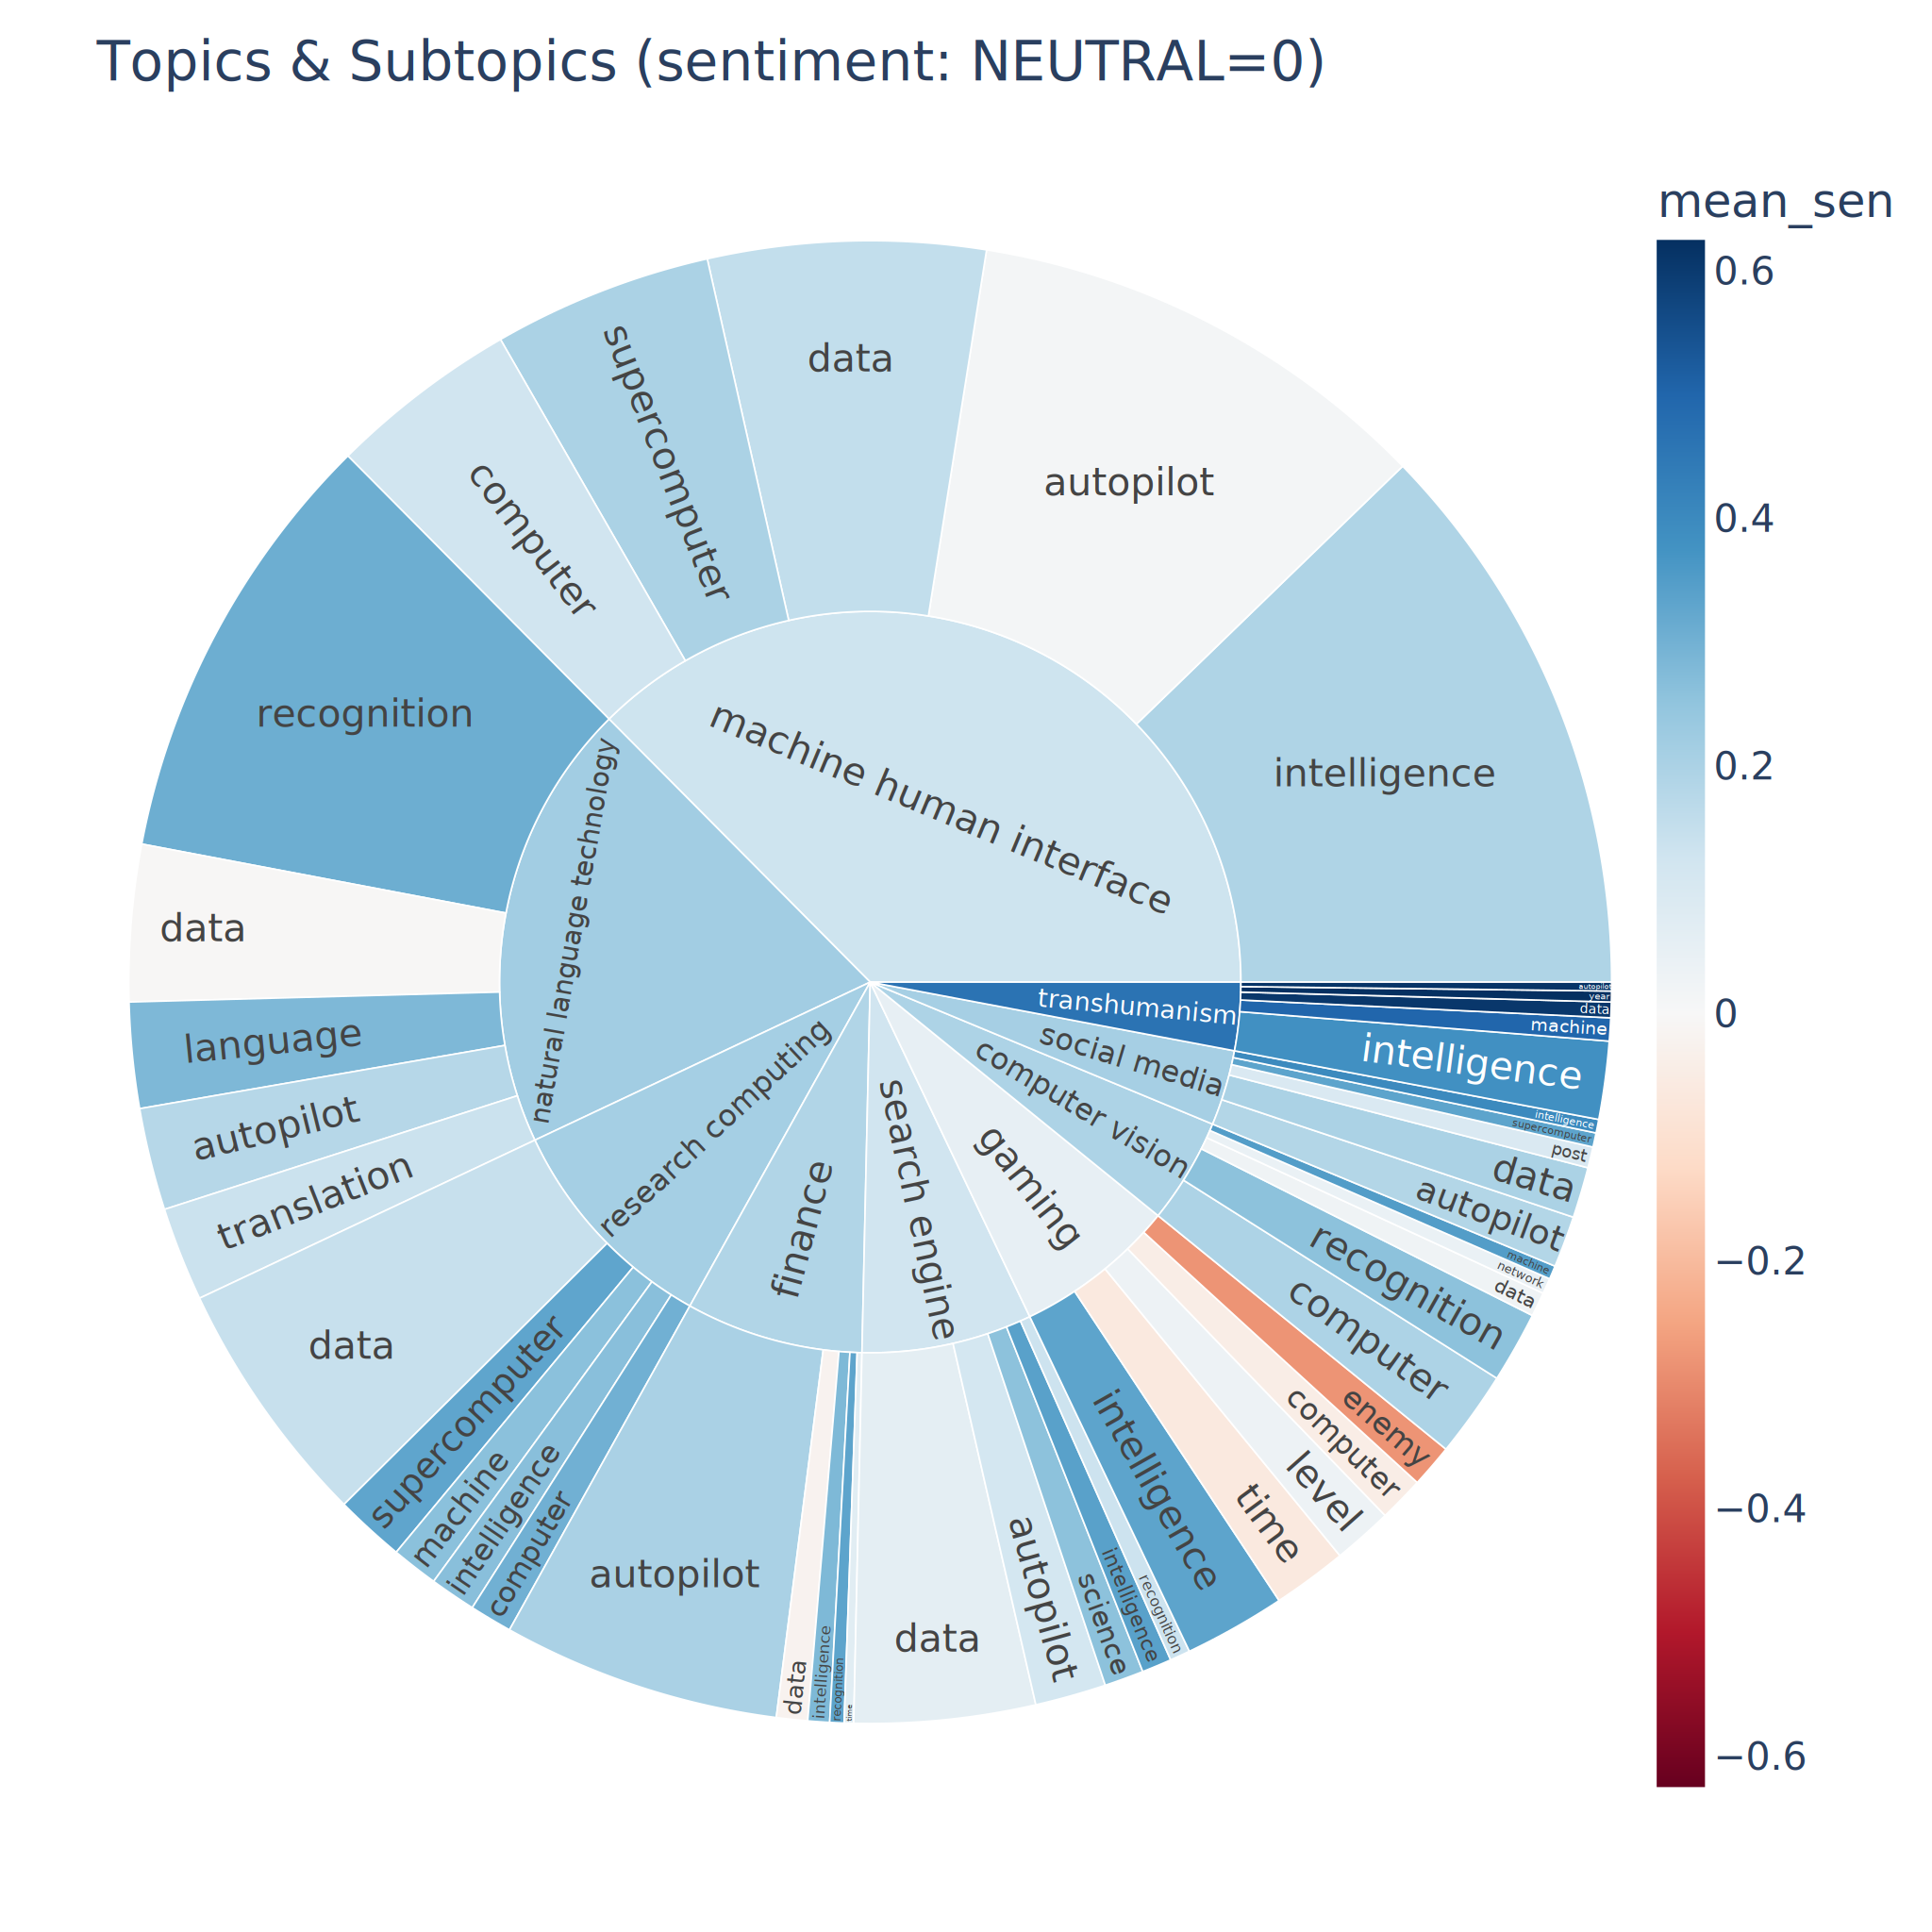
\includegraphics[width=0.6\textwidth]{pie_topics_subtopics_by_occ_sent_neu}
    \caption{
        Distribution of statements among the 9 topics (inner circle) and the most frequently occuring subtopic categories (outer circle).
        The Colorpalette (on the right) represents the average sentiment score of topics and subcategories (Red: NEGATIVE, White: NEUTRAL, Blue: POSITIVE).
        The majority of the average sentiment in both topics and subcategories is neutral.
    }
    \label{fig:pie_topics_subtopics_by_occ_sent_neu}
\end{figure}


\end{document}
